\documentclass{GSHS-chemexp}

\title{물의 증기압과 증발 엔탈피}	
\date{2016년 1월 11일 (월)}
\author{14088 이주찬}
\coauthor{14088 이주찬, 14088 이주찬}
	
\begin{document}

	\maketitle
	
	\section{실험 개요}
	
	\subsection{실험 목적}
	
	\begin{itemize}
		\item 온도에 따른 물의 증기압을 실험으로 측정한다.
		\item 측정 결과를 이용하여 물의 증발 엔탈피를 구한다.
	\end{itemize}
	
	\subsection{이론적 배경}
	
	\begin{itemize}
		\item {\bf 증기압} \\*
		증기가 고체 또는 액체와 동적 평형 상태에 있을 때 증기의 압력을 의미한다. 포화증기압, 증기 장력이라고도 한다. 증기압은 어떠한 액체의 증발속도와 관련이 있기 때문에, 실온 상태에서 증기압이 매우 높은 액체상태의 물질은 휘발성을 갖는 물질이라고 표현되기도 한다. 증기압은 같은 물질이라도 온도가 높아짐에 따라 더욱 커진다.
		\item {\bf 증발 엔탈피} \\*
		증발에 따른 엔탈피 변화. 정압에서의 증발열 또는 기화열과 같고, 그 물질의 기체상태와 액체상태의 엔탈피 차를 나타낸다.
		\begin{gather*}
			\mathrm{liquid} \rightleftarrows \mathrm{vap} \\
			K_{\mathrm{eq}} = P_{\mathrm{vap}} \\
			\ln \frac{P_{\mathrm{vap}}}{p^{\circ}} = \frac{\Delta H_{\mathrm{vap}}}{RT} + C
		\end{gather*}
		($P_{\mathrm{vap}}$ : 증기압, $p^{\circ}$ : 표준 압력, $\Delta H_{\mathrm{vap}}$ : 액체의 증발 엔탈피, $R$ : 기체 상수, $T$ : 절대 온도, $C$ : 상수)
		\begin{itemize}
			\item {\bf 증발 엔탈피 식의 유도} \\*
			$\Delta G^{\circ} = -RT \ln K$라는 식과 깁스 자유 에너지의 정의 $G = H - TS$로부터 $\Delta G^{\circ} = \Delta H^{\circ} - T \Delta S^{\circ}$임을 알 수 있다. \\
			위의 두 식을 연결하면, $\ln K = -\frac{\Delta H^{\circ}}{RT} + \frac{\Delta S^{\circ}}{R}$이 된다.
			물이 증발하는 경우 \ce{H_{2}O(l) <--> H_{2}O(g)}이고 열역학 평형 상수 $K = \frac{P_{\ce{H_{2}O}}}{p^{\circ}}$이다. 이 평형 상수 $K$를 대입하여 다시 정리하면 다음의 식을 얻을 수 있다.
			\begin{gather*}
				\ln \frac{P}{p^{\circ}} = -(\Delta H^{\circ}/RT) + \Delta S^{\circ}/R \ce{->} \ln \frac{P_{\mathrm{vap}}}{p^{\circ}} = -\frac{\Delta H_{\mathrm{vap}}}{RT} + C
			\end{gather*}
		\end{itemize}
		
		\item {\bf 유체 정지 압력} \\*
		자유 수면 아래에 정지해 있는 작은 정육면체 모양의 물을 생각해 보면, 정육면체 위의 물의 무게는 정육면체의 압력에 의해 평형을 이루어야 한다. 무한히 작은 정육면체를 생각하면, 이 무게, 즉 유체 정지압력은 다음과 같이 표현될 수 있다.
		\begin{gather*}
			P = \rho gh
		\end{gather*}
		($P$ : 유체 정지 압력, $\rho$ : 물의 밀도, $g$ : 중력 가속도, $h$ : 정육면체에서 자유 수면까지의 높이) \\
		일반적으로 유체의 밀도는 온도의 함수이고, 압축성 유체의 경우에는 압력의 함수가 된다.
		
	\end{itemize}
	
	\subsection{유의 사항}
	\begin{itemize}
		\item 눈금 실린더를 수직으로 하여 눈금을 읽는다. 또한, 한 명의 실험자가 일관된 기준으로 눈금을 읽는다.
		\item 실린더 내부의 공기 온도가 비커 내 물의 온도와 일치한다는 것을 전제할 수 있도록 눈금 실린더가 항상 물에 잠겨 있도록 한다.
		\item 온도 변화에 시간이 많이 소요되므로 집중한다. 온도를 낮출 때에는 얼음을, 높일 때에는 물을 넣어 온도를 빠르게 변화시키면 실험을 더 빨리 진행할 수 있지만 눈금 실린더 내의 공기와 물이 온도 평형을 이루어 같은 온도임을 가정하는 실험이므로 측정 온도 근처 부근에서는 자연히 온도가 올라가거나 내려갈 때까지 기다리는 것이 좋다.
	\end{itemize}
	
	\section{기구 및 시약}
	
	\subsection{실험 기구}
	기압계, \SI{2000}{\milli\litre} 비커, \SI{10}{\milli\litre} 눈금 실린더, 온도계, 가열판, \SI{30}{\centi\metre} 자
	\begin{itemize}
		\item {\bf 가열판} \\*
		가열판의 온도가 높아져도 겉으로 보이기에 큰 차이가 없어 화상을 입을 수 있으므로 주의한다. 온도 차 때문에 비커가 깨질 수 있으므로 찬 물이 든 비커를 뜨거워진 가열판에 바로 가열하지 않도록 한다.
		\item {\bf 기압계} \\*
		기압계를 실험 전에 미리 켜 두어야 한다. \\
		\sout{굳이 쓸 필요 없긴 한데 일단 두 개 이상의 예시가 필요해서 넣음}
	\end{itemize}
	\subsection{실험 시약}
	물
	\begin{itemize}
		\item {\bf 물} \\*
		호흡기에 다량 노출 시 폐가 치명적으로 손상되어 사망에 이를 수 있다. \\
		\sout{사실 별로 안 위험한데 일단 예시가 필요해서 넣음}
	\end{itemize}
	
	\section{실험 과정}
	
	\subsection{물의 증기압 측정}
	\begin{enumerate}
		\item 기압계에서 실험실의 대기압을 읽어 기록한다.
		\item \SI{2000}{\milli\litre} 비커를 물로 채운다.
		\item \SI{10}{\milli\litre} 눈금 실린더에 \SI{10}{\milli\litre} 눈금까지 물을 채운 후 손가락으로 막은 상태에서 신속히 비커 안에 뒤집어 세운다. 이때 눈금 실린더가 수직으로 안정되게 고정되도록 하고, 뒤집어 세웠을 때 공기 부분의 눈금이 \SI{4}{\milli\litre} 정도가 되어야 한다.
		\item 눈금 실린더가 물에 완전히 잠기도록 비커에 물을 보충한다.
		\item 비커 안에 온도계를 설치하고 가열판을 이용하여 \SI{80}{\degreeCelsius}까지 가열한다.
		\item 온도가 올라가면 가열판을 제거하고 \SI{80}{\degreeCelsius}부터 \SI{5}{\degreeCelsius} 간격으로 온도와 실린더의 수위를 읽고 기록하되, 공기 부분이 실린더 눈금 밖으로 벗어나지 않았는지 확인한다.
		\item 온도가 \SI{50}{\degreeCelsius} 아래로 떨어지면 얼음을 집어넣어 \SI{5}{\degreeCelsius} 아래가 될 때까지 온도를 신속히 떨어뜨린다. 이 과정에서 눈금 실린더의 눈금은 측정하지 않는다.
		\item 상온에 방치하면서 \SI{5}{\degreeCelsius} 부터 \SI{5}{\degreeCelsius} 간격으로 온도와 실린더의 수위를 읽고 기록한다.
		\item 실험 데이터로 실험 보고서에 절대 온도에 따른 수면 눈금을 표로 작성한다.
		\item \SI{5}{\degreeCelsius} 의 증기압은 무시하고, 측정한 실린더의 부피는 모두 공기로만 채워져 있다고 가정하여 각 온도에서의 공기압 $P_{\mathrm{air}}$를 구한다.
		\begin{gather*}
			P_{\mathrm{air}} = \frac{P_{\mathrm{air,~\SI{5}{\degreeCelsius}}} \cdot V_{\mathrm{air,~\SI{5}{\degreeCelsius}}}}{V_{\mathrm{air}}(T) \times \SI{278.15}{\kelvin}} \times T
		\end{gather*}
		\item 각 온도에서 얻어진 $P_{\mathrm{air}}$를 이용하여 분압 법칙으로부터 $P_{\mathrm{vap}}$를 구한다.
		\begin{gather*}
			P_{\mathrm{vap}} = P_{\mathrm{tot}} - P_{\mathrm{air}}
		\end{gather*}
		($P_{\mathrm{tot}}$ : 측정한 대기압)
		\item 각 온도에서의 $\ln P_{\mathrm{vap}}$를 구하고 $\ln P_{\mathrm{vap}}$ 대 $\frac{1}{T}$ 그래프를 그린다.
	\end{enumerate}
	\begin{figure}[H]
		\centering
		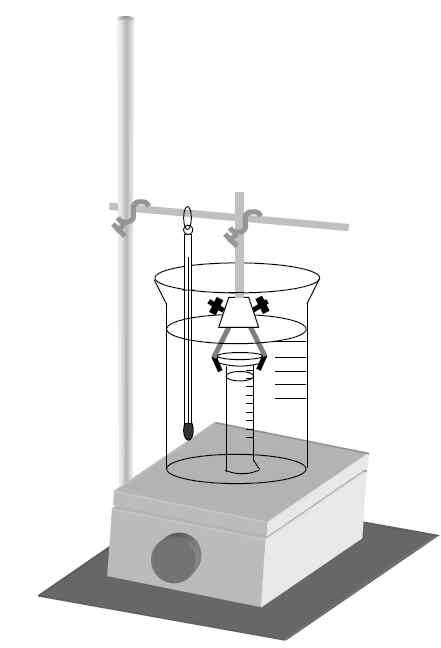
\includegraphics[width=0.3\textwidth]{expdiagram.png}
		\caption{실험 장치 모식도}
		\label{exp_diag}
	\end{figure}
	
	\section{실험 결과}
	
	\subsection{물의 증기압 측정}
	측정한 대기압은 다음과 같다.
	\begin{itemize}
		\item 대기압(\si{\kilo\pascal}) : 101.757
	\end{itemize}
	측정한 온도에 따른 눈금 실린더의 눈금, 그리고 실험 과정의 방법을 이용하여 계산한 증기압을 \ref{table_vap}에 나타내었다.
	
	\begin{table}[H]
		\centering
		\begin{tabular}{D..{2.1} D..{2.2} D..{1.4}}
			\hline
			\multicolumn{1}{c}{온도(\si{\degreeCelsius})} & %
			\multicolumn{1}{c}{눈금(\si{\milli\metre})} & %
			\multicolumn{1}{c}{증기압(\si{\atmosphere})} \\
			\hline \hline
			80.0	& 10.00	& 0.4954	\\
			75.0	& 8.22	& 0.394		\\
			70.0	& 7.15	& 0.313		\\
			65.0	& 6.41	& 0.244		\\
			60.0	& 6.00	& 0.204		\\
			55.0	& 5.61	& 0.161		\\
			50.0	& 5.31	& 0.127		\\
			20.0	& 4.31	& 0.0243	\\
			15.0	& 4.21	& 0.0181	\\
			10.0	& 4.12	& 0.0140	\\
			5.0		& 3.99	& \approx 0	\\
			\hline
		\end{tabular}
		\caption{온도에 따른 눈금 실린더의 눈금과 그를 통해 계산한 증기압 표}
		\label{table_vap}
	\end{table}
	
	절대 온도의 역수와 증기압의 자연로그 값을 이용하여 그린 그래프는  \ref{exp_graph}\와 같다.
	
	\begin{figure}[H]
		\centering
		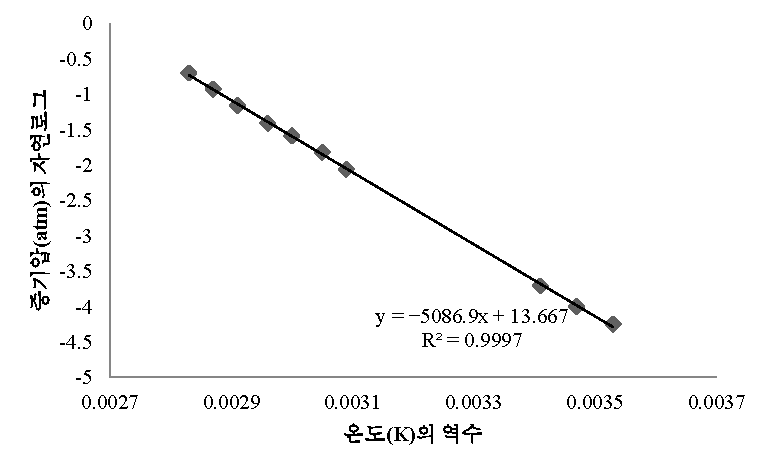
\includegraphics[scale=1]{Book3.pdf}
		\caption{절대 온도의 역수와 증기압의 자연로그 값의 그래프}
		\label{exp_graph}
	\end{figure}
	
	선형 추세선의 식은 $y = -5086.9x + 13.667$이다.
	실험을 할 때 눈금 실린더 안의 수면은 비커의 수면보다 낮은 위치에 있다. 따라서 압력을 구할 때에는 이를 보정하는 것이 필요하다. 수면과 비커의 높이 차를 이용, $P = \rho gh $식을 이용하여 수압을 더해 주어야 눈금 실린더 내의 기체 압력을 알 수 있다. 실험 과정에서 얼음, 물 등을 넣거나 빼어 비커의 수면 높이가 달라지므로 측정 시마다 높이 차를 측정하였다. 온도에 따른 높이 차와 이를 고려하여 다시 구한 증기압을 \ref{table_vap_2}에 나타내었다.
	
	
	\begin{table}[H]
		\centering
		\begin{tabular}{D..{2.1} D..{2.2} D..{1.5}}
			\hline
			\multicolumn{1}{c}{온도(\si{\degreeCelsius})} & %
			\multicolumn{1}{c}{눈금(\si{\milli\metre})} & %
			\multicolumn{1}{c}{증기압(\si{\atmosphere})} \\
			\hline \hline
			80.0	& 10.50	& 0.4878	\\ 
			75.0	& 9.20	& 0.387		\\ 
			70.0	& 8.05	& 0.307		\\ 
			65.0	& 7.54	& 0.238		\\ 
			60.0	& 7.09	& 0.199		\\ 
			55.0	& 6.89	& 0.156		\\ 
			50.0	& 6.94	& 0.121		\\ 
			20.0	& 5.43	& 0.0193	\\ 
			15.0	& 5.39	& 0.0131	\\ 
			10.0	& 5.31	& 0.00914	\\ 
			5.0		& 5.20	& \approx 0	\\ 
			\hline
		\end{tabular}
		\caption{온도에 따른 수면과의 높이 차와 이로 보정한 증기압 표}
		\label{table_vap_2}
	\end{table}
	
	절대 온도의 역수와 보정한 증기압의 자연로그 값을 이용하여 그린 그래프는 \ref{exp_graph_2}\과 같다.
	
	\begin{figure}[H]
		\centering
		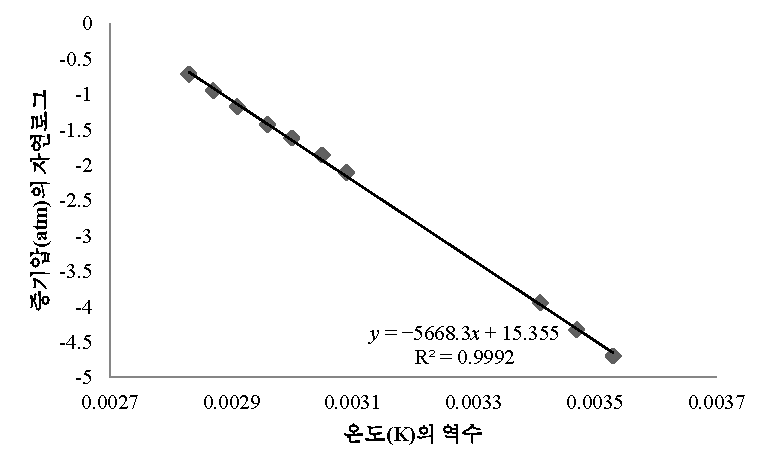
\includegraphics[scale=1]{Book3_2.pdf}
		\caption{절대 온도의 역수와 보정한 증기압의 자연로그 값의 그래프}
		\label{exp_graph_2}
	\end{figure}
	
	보정 값을 이용한 선형 추세선의 식은 $y = -5668.3x + 15.355$이다.
	
	\section{관찰 및 토의}
	
	\subsection{수압 보정}
	실험을 할 때 눈금 실린더 안의 수면은 비커의 수면보다 낮은 위치에 있다. 따라서 압력을 구할 때에는 이를 보정하는 것이 필요하다. 수면과 비커의 높이 차는 \SI{5}{\centi\metre} - \SI{10}{\centi\metre} 정도였고 이를 보정하면 약 \SI{0.005}{\atmosphere} - \SI{0.01}{\atmosphere} 정도의 오차를 나타내게 된다. 높은 온도에서는 이러한 오차가 크지 않겠지만 낮은 온도에서는 이 정도의 오차가 계산한 증기압의 수 십 퍼센트나 된다. 실제로 위 실험 결과에서 구한 증기압과 그 추세선의 식은 상당한 차이를 보였음을 볼 수 있었다.
	
	\subsection{메니스커스 보정}
	실험에서 눈금을 읽을 때, 메니스커스의 아래 눈금을 읽으면 그 윗부분에도 물이 있기 때문에 실제 부피보다 더 큰 값으로 읽게 된다. 따라서 일정 값을 기체 부피에서 빼 주어 메니스커스 보정을 해 주어야 한다. 본 실험에서는 이러한 특성을 고려하여 눈금을 메니스커스의 눈금 중앙으로 읽어 정확한 부피에 최대한 가까운 값을 사용하려 하였다.
	
	\subsection{실험에서 순수한 공기의 분압을 구하는 과정에 있어서 사용한 가정}
	\begin{itemize}
		\item \SI{5}{\degreeCelsius}에서 물의 증기압은 0이다. \\
		실험 결과를 산출할 때 \SI{5}{\degreeCelsius}에서 물의 증기압을 0으로 가정하고 계산하였다. 그러나 실제로 \SI{5}{\degreeCelsius}의 증기압은 약 \SI{0.0086}{\atmosphere}이고, 이 때문의 저온의 값들은 실제 증기압보다 더 큰 값으로 구해져 증발 엔탈피를 더 작게 만든다.
		\item 공기는 이상 기체와 유사한 성질을 지닌다(이상 기체처럼 행동한다).
		기본적인 이상 기체 상태 방정식 $PV=nRT$를 쓰기 위해서라도 이러한 가정을 하여야 하며, 이는 타당한 가정이라고 보아도 무방하다.
		\item 증발 엔탈피와 증발 엔트로피는 온도에 따라서 변하지 않는다. \\
		실제 물의 증발 엔탈피는 끓는점인 \SI{100}{\degreeCelsius}에서는 약 \SI{41}{\kilo\joule\per\mole}이지만 \SI{0}{\degreeCelsius}에서는 약 \SI{45}{\kilo\joule\per\mole}이다.\cite{vapor_1} 따라서 낮은 온도에서의 실험 자료는 그만큼 계산한 증발 엔탈피 값을 크게 할 것이다.
		
	\end{itemize}
	
	\subsection{물의 증발 엔탈피}
	문헌의 물의 증발 엔탈피 값은 \SI{40.66}{\kilo\joule\per\mole}이다. \cite{vapor_1} \\
	실험을 통해 그린 그래프의 추세선 식은 $y = -5668.3x + 15.355$이었다. $x$의 계수를 $-a$라 한다면 $\ln P_{\mathrm{vap}} = -\frac{\Delta H_{\mathrm{vap}}}{RT} + C$ 식에서 $\Delta H_{\mathrm{vap}} = aR$로 증발 엔탈피를 구할 수 있다. 따라서 이를 통해 계산한 물의 증발 엔탈피는 다음과 같다.
	\begin{itemize}
		\item 물의 증발 엔탈피(\si{\kilo\joule\per\mole}) : 47.1
	\end{itemize}
	
	\subsubsection{저온에서의 측정값}
	실험을 진행할 때, 낮은 온도에서는 부피의 변화량도 적고, 이에 따라 측정도 그만큼 어려워지게 된다. \SI{0.1}{\milli\litre} 남짓 변하는 변화를 정확하게 관찰하지 못한다면 그만큼 실험 결과에는 큰 오차를 불러일으킬 것이다. 예를 들어, 이번 실험 데이터에서 \SI{10}{\degreeCelsius}의 부피를 \SI{4.12}{\milli\litre}가 아닌 \SI{4.13}{\milli\litre}로 측정했다면 추세선 그래프의 계수는 각각 -5086.9, -5668.3에서 -4984.2, -5504.0으로 변한다. 따라서 저온에서의 값을 신뢰하기에는 무리가 따르고, \SI{10}{\degreeCelsius}에서 \SI{20}{\degreeCelsius}까지의 값을 무시한 채로 온도의 역수와 보정한 증기압의 자연로그 값의 그래프를 다시 그린 그래프는 \ref{exp_graph_3}\와 같다.
	
	\begin{figure}[H]
		\centering
		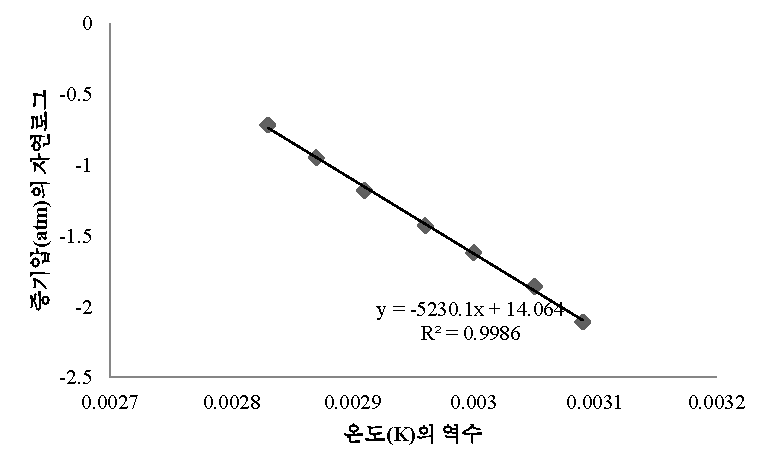
\includegraphics[scale=1]{Book3_3.pdf}
		\caption{\SI{10}{\degreeCelsius}에서 \SI{20}{\degreeCelsius}까지의 값을 무시하여 그린\\절대 온도의 역수와 보정한 증기압의 자연로그 값의 그래프}
		\label{exp_graph_3}
	\end{figure}
	
	추세선의 계수는 -5230.1이 되었고, 이를 이용하여 다시 구한 물의 증발 엔탈피는 다음과 같다.
	\begin{itemize}
		\item 물의 증발 엔탈피(\si{\kilo\joule\per\mole}) : 43.5
	\end{itemize}
	
	\subsection{물의 정상 끓는점}
	$\ln P_{\mathrm{vap}} = -\frac{\Delta H_{\mathrm{vap}}}{RT} + C$ 식을 이용, 기울기를 $y$ 절편으로 나누어 주면 물의 끓는점을 구할 수 있다. 이에 따른 물의 끓는점은 다음과 같다.
	\begin{itemize}
		\item 물의 끓는점(\si{\degreeCelsius}) : 99
	\end{itemize}
	이는 이론적 끓는점인 \SI{100}{\degreeCelsius}와 약간의 차이를 보인다. 이는 $\Delta H$와 $\Delta S$를 일정하다고 가정하고 값을 구했는데 실제로는 온도에 따라 그 값이 변하므로 오차가 발생했을 것이다.
	
	\section{결론 및 제언}
	증기압 측정에서, 저온의 경우 부피 변화가 크지 않아 작은 측정 오차도 결과 값에 큰 영향을 미치게 되고, 최저온 측정값을 0으로 가정하는 것 역시도 큰 오차를 만들어낸다. 따라서, 여러 온도에서 증기압을 측정하여 증발 엔탈피와 정상 끓는점을 결정할 때에는 증기압 변화가 큰 높은 온도에서 실험하는 것이 좋다.
	
	
	\begin{thebibliography}{00}
		\bibitem{vapor_2} David R. Lide, ed. (2005), \textit{CRC Handbook of Chemistry and Physics}. Boca Raton, Florida: CRC Press
		\bibitem{vapor_1} Marsh, K. N., Ed., \textit{Recommended Reference Materials for the Realization of Physicochemical Properties}, Blackwell, Oxford, 1987 %%일반화학실험 교재에 값이 있으니 그걸로 수정하는 것이 좋을 것 같다.
	\end{thebibliography}
			
\end{document}